\chapter{Programmazione greedy}
Gli algoritmi realizzati per risolvere \emph{problemi di ottimizzazione}
eseguono una sequenza di decisioni che, nel caso della \emph{programmazione
dinamica}, sono prese in maniera bottom-up valutando tutte le possibilità,
evitando però di ripetere decisioni già esaminate. Con la \emph{programmazione
greedy} invece, tra tutte le possibili decisioni ne viene scelta solo una,
quella che sembra ottima, o meglio localmente ottima. Tuttavia, è necessario
dimostrare che quella particolare scelta permette di ottenere un risultato
ottimo anche a livello globale.

Proprio per questo motivo, la \emph{programmazione greedy} è utilizzabile sono
per quei problemi che presentano una \emph{sottostruttura ottima} e per i
quali è possibile dimostrare che esiste una scelta \q{ingorda}, cioè una scelta
che porta ad una soluzione ottima.

\section{Problema del resto}
\begin{problem}[Problema del resto]
    Dati un insieme di \q{tagli} di monete, espressi come un vettore $t[1\dots n]$
    di interi positivi, e un valore $R$ rappresentate un resto da dover restituire,
    trovare il più piccolo numero intero di pezzi necessari per dare un resto
    $R$ di centesimi, utilizzando i tagli disponibili e assumendo di avere un
    numero illimitato di monete.

    Formalmente, è necessario trovare un vettore $x$ di interi non negativi
    tale per cui:
    \[R=\sum_{i=1}^n x[i]\cdot t[i]\quad\text{e}\quad m=\sum_{i=1}^n x[i]\quad
    \text{ha valore minimo}\]
\end{problem}

\noindent
Questo problema possiede una \emph{sottostruttura ottima}:
\begin{definition}[Sottostruttura ottima]
    Siano $S(i)$ il problema di dare un resto pari ad $i$ e $A(i)$ una soluzione
    ottima del problema $S(i)$ rappresentata da un multi-insieme. Sia poi
    $j\in A(i)$. Allora, $S(i-t[j])$ è un sotto-problema di $S(i)$, la cui
    soluzione è data da $A(i)-\{j\}$.
\end{definition}

\subsection{Approccio basato su programmazione dinamica}
Prima di vedere come potrebbe essere realizzata una soluzione \emph{greedy},
utilizziamo le proprietà della \emph{sottostruttura ottima} per implementare
una soluzione basata su \emph{programmazione dinamica}.

\noindent
Se $DP[i]$ rappresenta il numero minimo di monete necessario a risolvere il
problema $S(i)$, vale la seguente funzione ricorsiva:
\[DP[i]=\begin{cases}
    0 & i=0\\
    \min_{1\leq j\leq n}\{DP[i-t[j]]\;|\;t[j]\leq i\}+1 & i>0
\end{cases}\]

\begin{minicode}{Soluzione basata su programmazione dinamica}
\ind\bc{int}[] moneyChange(\bc{int}[] t, \bc{int} n, \bc{int} R)\\
    \bc{int}[] DP = new \bc{int}[0\dots R]\hfill\com{\emph{Tabella delle soluzioni}}
    \bc{int}[] coins = new \bc{int}[0\dots R]\hfill\com{Moneta da usare per uno specifico resto}
    DP[0] = 0\\
    \indf for (i = 1 to R) do\\
        DP[i] = $+\infty$\\
        \indff for (j = 1 to n) do\\
            \indfff if (i > t[j] and DP[i - t[j]] + 1 < DP[i]) then\\
                DP[i] = DP[i - t[j]] + 1\\
                coins[i] = j\\
    \indf\com{Ricostruzione della soluzione}
    \indf\bc{int}[] x = new \bc{int}[1\dots n] = \{0\}\hfill\com{Contatore delle monete usate}
    \indf while (R > 0) do\\
        x[coins[R]] = x[coins[R]] + 1\\
        R = R - t[coins[R]]\\
    \indf return x
\end{minicode}

\paragraph{Complessità}
La \emph{complessità} di questa soluzione è $\Theta(nR)$ per la presenza dei
due cicli annidati.

\subsection{Approccio basato su programmazione greedy}
Non è difficile immaginare che per minimizzare il numero di monete utilizzate
sia sufficiente usare sempre il taglio più grande possibile. Ovvero, selezionare
la moneta $j$ più grande, tale per cui $t[j]\leq R$, e risolvere il sotto-problema
$S(R-t[j])$.

\begin{minicode}{Soluzione basata su programmazione greedy}
\ind\bc{int}[] moneyChange(\bc{int}[] t, \bc{int} n, \bc{int} R)\\
    \bc{int}[] x = new \bc{int}[1\dots n]\\
    \{ \text{Ordina le monete in modo decrescente} \}\\
    \indf for (i = 1 to n) do\\
        x[i] = $\lfloor$R / t[i]$\rfloor$\\
        R = R - x[i] $\cdot$ t[i]\\
    \indf return x
\end{minicode}

\paragraph{Complessità}
Questa soluzione abbassa la \emph{complessità} a $O(n\log n)$ se l'insieme di
monete non è ordinato, $O(n)$ altrimenti.

\bigskip\noindent
Ciò che dobbiamo fare adesso è dimostrare che la scelta fatta sia corretta.

\begin{proof}[Dimostrazione]
    Supponiamo $t=[50, 10, 5, 1]$. Sia $x$ una qualunque soluzione ottima, ovvero
    tale per cui:
    \[R=\sum_{i=1}^n x[i]\cdot t[i]\quad\text{e}\quad m=\sum_{i=1}^n x[i]\quad
    \text{ha valore minimo}\]
    Sappiamo che $t[k]\cdot x[k]<t[k-1]$ altrimenti basterebbe sostituire un certo
    numero di monete di taglio $t[k]$ con quelle del taglio $t[k-1]$. In questo
    caso, i limiti al numero di monete per ogni taglio sono:
    \[\begin{array}{rclccclcl}
        t[2]\cdot x[2] & = & 10\cdot x[2] & < & t[1] & = & 50 & \Rightarrow & x[2]<5\\
        t[3]\cdot x[3] & = & 5\cdot x[3] & < & t[2] & = & 10 & \Rightarrow & x[3]<2\\
        t[4]\cdot x[4] & = & 1\cdot x[4] & < & t[3] & = & 5 & \Rightarrow & x[4]<5\\
    \end{array}\]
    Sia ora $m_k$ la somma delle monete di taglio inferiore a $t[k]$:
    \[m_k=\sum_{i=k+1}^4 x[i]\cdot t[i]\]
    Se riusciamo a dimostrare che $m_k<t[k]$ $\forall k$, allora la soluzione
    proposta dall'algoritmo è proprio quella ottima. Per ogni valore di $k$
    otteniamo:
    \[\begin{array}{rclclclclc}
        m_4 & = & 0 & & & < & 1 & & & =t[4]\\
        m_3 & = & x[4]\cdot1+m_4 & \leq & 4\cdot 1+m_4 & < & 4+1 & = & 5 & =t[3]\\
        m_2 & = & x[3]\cdot1+m_3 & \leq & 1\cdot 5+m_3 & < & 5+5 & = & 10 & =t[2]\\
        m_1 & = & x[2]\cdot1+m_2 & \leq & 4\cdot 10+m_2 & < & 40+10 & = & 50 & =t[1]\\
    \end{array}\]
\end{proof}
\begin{note}
    Non tutti i tagli di monete permettono di utilizzare la \emph{programmazione
    greedy}. Ad esempio, per $t[10,8,1]$ l'algoritmo \emph{greedy} utilizzerebbe
    una moneta da 10 e 7 da 1, quando la scelta migliore sarebbe quella di
    prenderne 2 da 8 e una da 1.
\end{note}
\begin{note}
    In ogni caso, l'insieme delle monete deve includere una moneta di taglio
    unitario.
\end{note}

\section{Insieme indipendente massimale di intervalli}
Vediamo un caso particolare del problema sulla \nameref{prob:12} in cui il peso
di tutti gli intervalli è $1$. Cioè, vogliamo cercare l'insieme contenente il
maggior numero di intervalli.

\begin{figure}[h!]
    \centering
    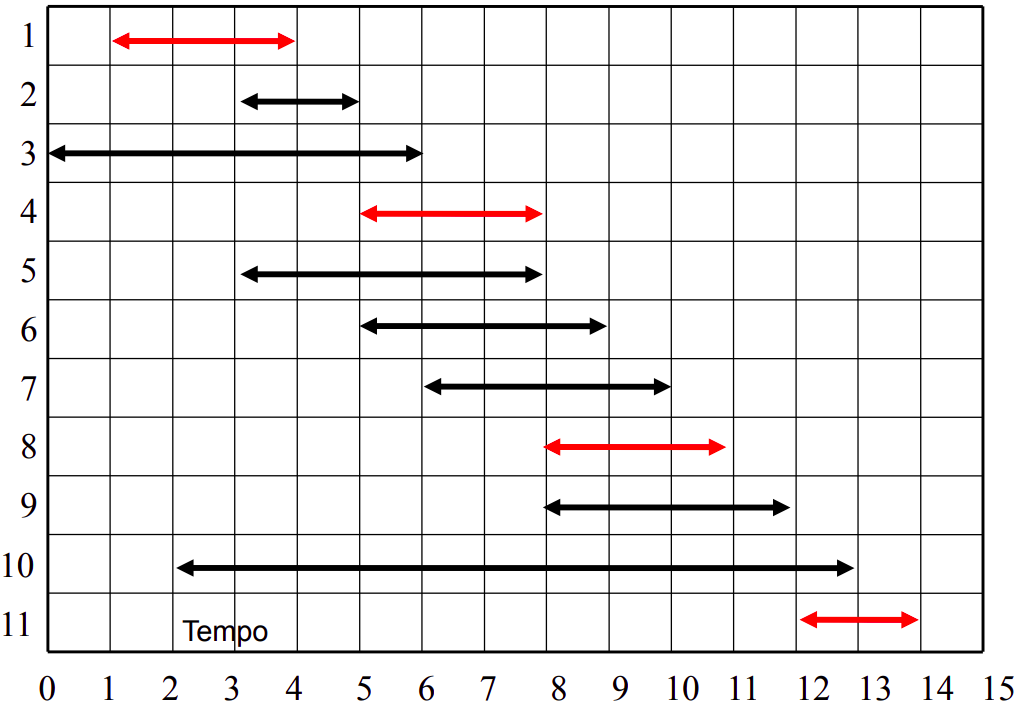
\includegraphics[width=0.45\textwidth]{intervalli-ordinati-greedy1.png}
    \caption{Possibile soluzione}
\end{figure}

\subsection{Approccio basato su programmazione dinamica}
Iniziamo ricercando una \emph{sottostruttura ottima}. Assumiamo che gli intervalli
siano ordinati per tempo di fine:
\[b_1\leq\dots\leq b_n\]
Definiamo il sotto-problema $S[i\dots j]$ come l'insieme di intervalli che
iniziano dopo la fine di $i$ e finiscono prima dell'inizio di $j$:
\[S[i\dots j]=\{k\;|\;b_i\leq a_k<b_k\leq a_j\}\]
Aggiungiamo due intervalli fittizi:
\begin{itemize}
    \item \emph{Intervallo $0$}: $b_0=-\infty$;
    \item \emph{Intervallo $n+1$}: $a_{n+1}=+\infty$;
\end{itemize}
Il problema generale corrisponde quindi al problema $S[0\dots n+1]$.

\begin{definition}[Sottostruttura ottima]
    Supponiamo che $A[i\dots j]$ sia una soluzione ottimale di $S[i\dots j]$
    e sia $k$ un intervallo che appartiene ad $A[i\dots j]$. Allora:
    \begin{itemize}
        \item Il problema $S[i\dots j]$ può essere suddiviso in due intervalli:
        \begin{enumerate}
            \item $S[i\dots k]$ contenente gli intervalli di $S[i\dots j]$ che
            finiscono prima di $k$;
            \item $S[k\dots j]$ contenente gli intervalli di $S[i\dots j]$ che
            iniziano dopo $k$;
        \end{enumerate}
        \item $A[i\dots j]$ contiene le soluzioni ottimali di $S[i\dots k]$ e
        $S[k\dots j]$:
        \begin{enumerate}
            \item $A[i\dots j]\cap S[i\dots k]$ è la soluzione ottimale di $A[i\dots k]$;
            \item $A[i\dots j]\cap S[k\dots j]$ è la soluzione ottimale di $A[k\dots j]$;
        \end{enumerate}
    \end{itemize}
\end{definition}

\noindent
Quanto detto ci permette di definire $A[i\dots j]$ come:
\[A[i\dots j]=A[i\dots k]\cup\{k\}\cup A[k\dots j]\]
Per determinare $k$ proviamo tutte le possibilità. A questo punto, sia $DP[i][j]$
la dimensione del più grande sottoinsieme $A[i\dots j]\subseteq S[i\dots j]$ di
intervalli indipendenti. Possiamo definire $DP[i][j]$ con la seguente funzione
ricorsiva:
\[DP[i][j]=\begin{cases}
    0 & S[i\dots j]=\emptyset\\
    \max_{k\in S[i\dots j]}\{DP[i][k]+DP[k][j]+1\} & \text{altrimenti}
\end{cases}\]
Questa definizione ci permette di realizzare un algoritmo basato su
\emph{programmazione dinamica}, o su \emph{memoization}, con \emph{complessità}
pari a $O(n^3)$. Questo perché bisogna risolvere tutti i problemi con $i<j$ e,
nel caso peggiore, paghiamo $O(n)$ per ogni sotto-problema.

\bigskip\noindent
Possiamo fare meglio di così?

Potremmo semplicemente usare la soluzione al problema con pesi generici, che
ha \emph{complessità} $O(n\log n)$, ponendo a $1$ tutti i pesi. Tuttavia,
potremmo anche chiederci se sia davvero necessario analizzare tutti i
possibili valori di $k$. Definiamo il seguente teorema:

\begin{definition}[Scelta ingorda]
    Siano $S[i\dots j]$ un sotto-problema non vuoto e $m$ l'intervallo di $S[i\dots
    j]$ con il minor tempo di fine. Allora, valgono i due seguenti punti:
    \begin{enumerate}
        \item Il sotto-problema $S[i\dots m]$ è vuoto;
        \item $m$ è compreso in una qualche soluzione ottima di $S[i\dots j]$,
        ovvero $m\in A[i\dots j]$;
    \end{enumerate}
\end{definition}
\begin{proof}[Dimostrazione]
    Dimostriamo separatamente i due punti.

    \paragraph{Punto 1 - \bm{$S[i$}\dots\bm{$ j]=\emptyset$}}
    Per la definizione di intervallo sappiamo che $a_m<b_m$. Inoltre, poiché $m$
    è l'intervallo con il minor tempo di fine, $\forall k\in S[i\dots j]$ $b_m
    \leq b_k$ e quindi, ne consegue che $\forall k\in S[i\dots j]$ $a_m<b_k$.
    Se nessun intervallo in $S[i\dots j]$ termina prima di $a_m$, allora $S[i
    \dots m]=\emptyset$.

    \paragraph*{Punto 2 - \bm{$m\in A[i$}\dots\bm{$i]$}}
    Siano $A'[i\dots j]$ una soluzione ottima di $S[i\dots j]$ e $m'$ l'intervallo
    con minor tempo di fine in $A'[i\dots j]$. Sia ora $A[i\dots j]=A'[i\dots j]
    -\{m'\}\cup\{m\}$ una nuova soluzione ottima ottenuta togliendo $m'$ e
    aggiungendo $m$ ad $A'[i\dots j]$. $A[i\dots j]$ è una soluzione ottima che
    contiene $m$ in quanto ha la stessa cardinalità di $A'[i\dots j]$ e gli
    intervalli sono indipendenti.
\end{proof}

\noindent
Questa dimostrazione ci permette di selezionare sempre gli intervalli con tempo
di fine minore e ignorare tutti quelli che si intersecano con esso, riducendo
il problema alla ricerca dell'\emph{insieme indipendente massimale} in $S[m\dots
j]$.

\begin{figure}[h!]
    \centering
    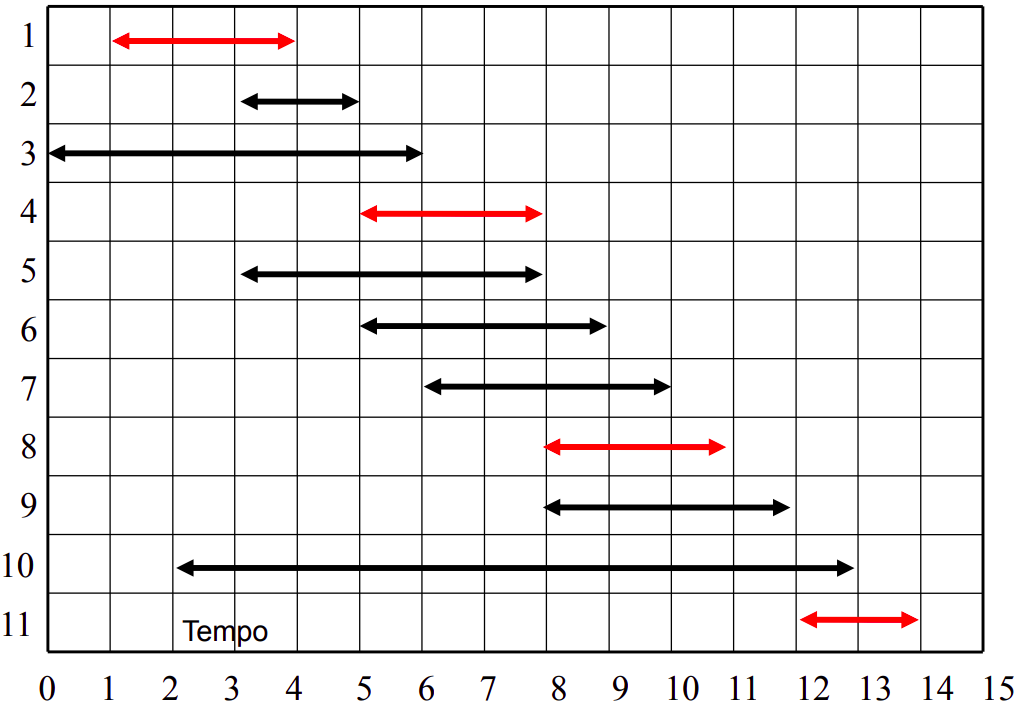
\includegraphics[width=0.45\textwidth]{intervalli-ordinati-greedy1.png}
    \caption{Soluzione con \emph{scelte ingorde}}
\end{figure}

\begin{minicode}{Soluzione basata su programmazione greedy}
\ind\bc{SET} indipendentSet(\bc{int}[] a, \bc{int}[] b)\\
    \{ Ordina i vettori $a$ e $b$ in modo che $b_1\leq\dots\leq b_n$ \}\\
    \bc{SET} S = Set()\\
    S.insert(1)\\
    \bc{int} last = 1\\
    \indf for (i = 2 to n) do\\
        \indff if (a[i] $\geq$ b[last]) then\\
            S.insert(i)\\
            last = i\\
    \indf return S
\end{minicode}

\paragraph{Complessità}
Questa soluzione abbassa la \emph{complessità} a $O(n)$ se i vettori di input
sono già ordinati, $O(n\log n)$ altrimenti.

\begin{eg}[Esempio d'esecuzione]
    Il comportamento del nuovo algoritmo con gli stessi intervalli degli esempi
    precedenti è il seguente:

    \begin{figure}[h!]
        \centering
        \subfloat{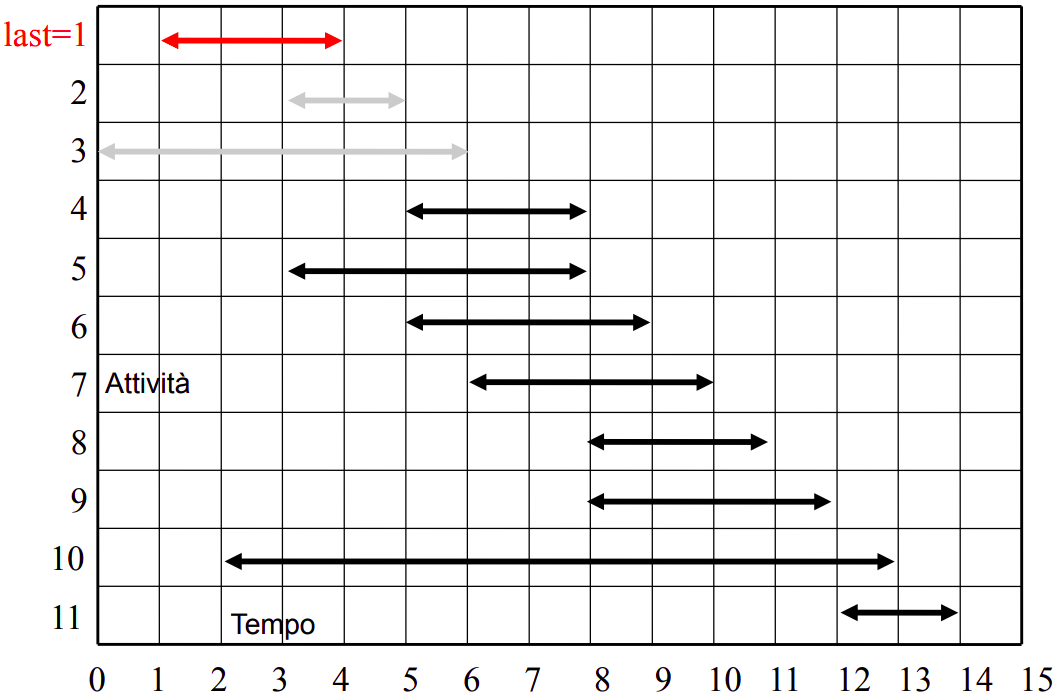
\includegraphics[width=0.48\textwidth]
        {intervalli-ordinati-greedy-s1.png}}
        \hfill
        \subfloat{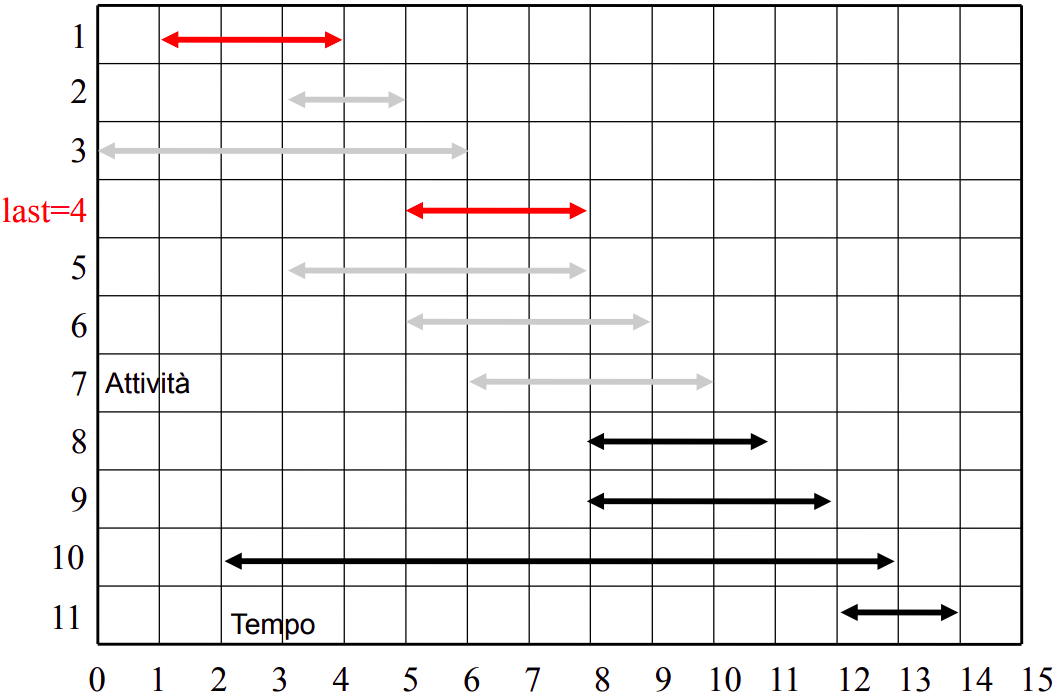
\includegraphics[width=0.48\textwidth]
        {intervalli-ordinati-greedy-s2.png}}\\
        \subfloat{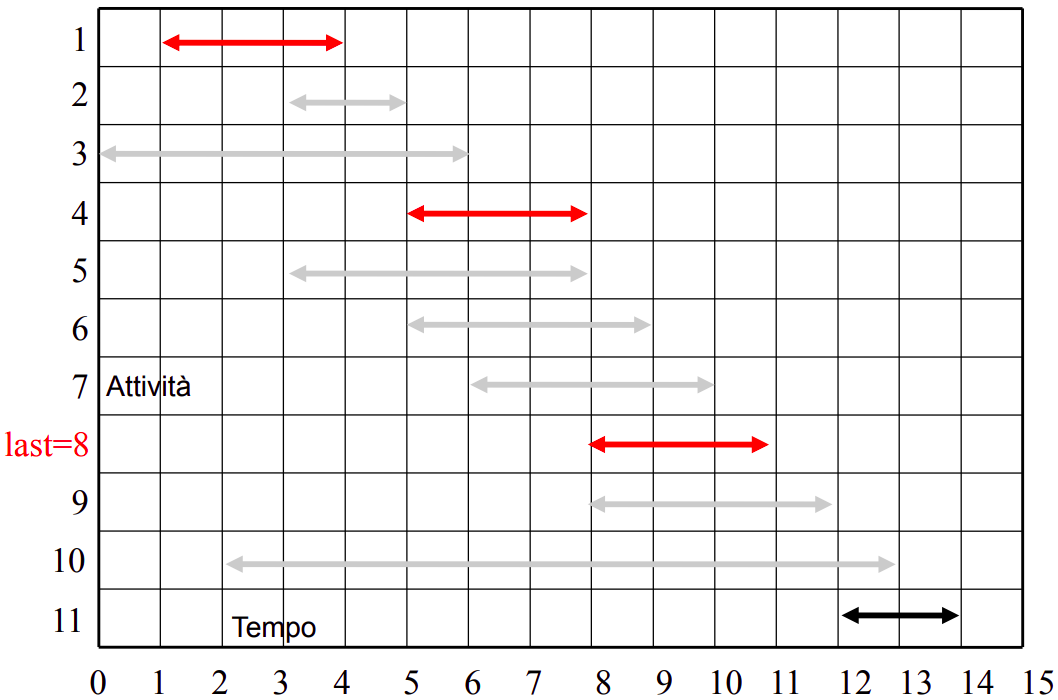
\includegraphics[width=0.48\textwidth]
        {intervalli-ordinati-greedy-s3.png}}
        \hfill
        \subfloat{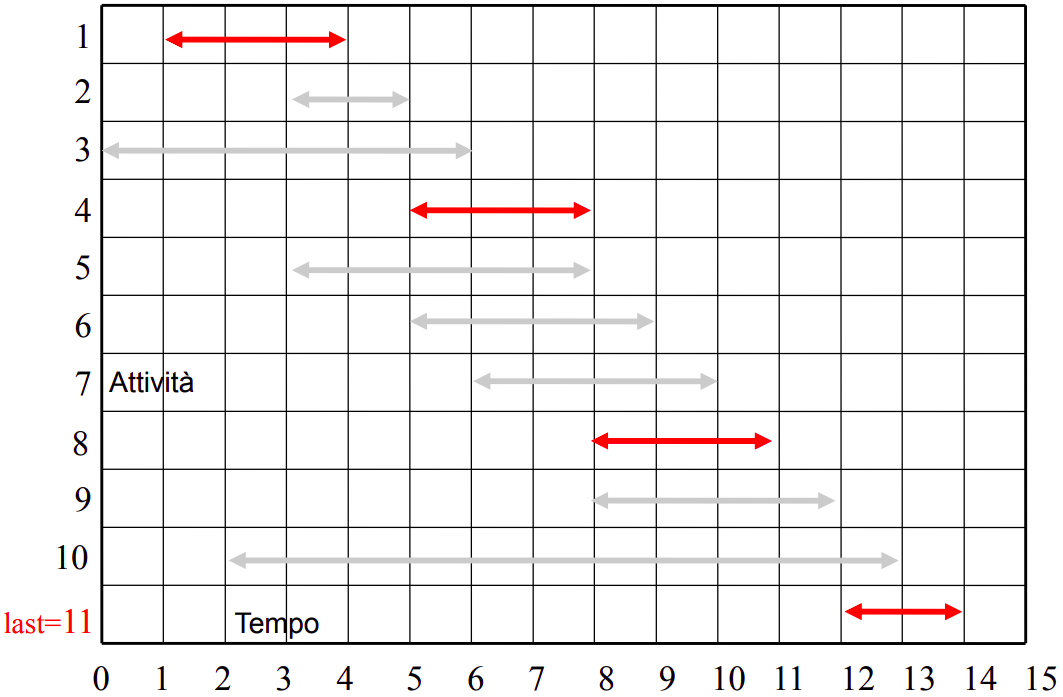
\includegraphics[width=0.48\textwidth]
        {intervalli-ordinati-greedy-s4.png}}
    \end{figure}
\end{eg}

\section{Problema dello scheduling}
\begin{problem}[Scheduling dei processi]
    Dati un processore e $n$ processi da eseguire su di esso. Se ogni processo $i$
    è caratterizzato da un tempo d'esecuzione $t[i]$ noto a priori, trovare una
    sequenza d'esecuzione che minimizzi il tempo di completamento medio.
\end{problem}
\begin{definition}[Tempo di completamento]
    Dato un vettore $A[1\dots n]$ contenente una permutazione di $\{1\dots n\}$,
    il tempo di completamento dell'$h$-esimo processo nella permutazione è
    calcolato come:
    \[T_A(h)=\sum_{i=1}^h t[A[i]]\]
\end{definition}

\newpage
\begin{eg}[Possibili permutazioni]
    Consideriamo i seguenti processi con relativo tempo d'esecuzione:
    
    \begin{table}[h!]
        \centering
        \renewcommand{\arraystretch}{1.2}
        \begin{tabular}{|c|c|c|c|c|}
            \hline
            \textbf{Processo} & $1$ & $2$ & $3$ & $4$\\
            \hline
            \bm{$t[i]$} & 4 & 1 & 6 & 3\\
            \hline
        \end{tabular}    
    \end{table}

    \noindent
    Se eseguissimo i processi nell'ordine $A[1,2,3,4]$ la situazione sarebbe
    la seguente:

    \begin{figure}[h!]
        \centering
        \begin{graph}
            \tikzset{
                cell/.style={rectangle, draw, minimum size=10mm, anchor=west},
            }
            \node[cell] (1) [minimum width=40mm, label={[xshift=-12mm]225:{$0$}}] {$4$};
            \node[cell] (2) [minimum width=10mm, right of=1, xshift=5mm,
            label={[xshift=3mm]225:{$4$}}, label={[xshift=-3mm]-45:{$5$}}] {$1$};
            \node[cell] (3) [minimum width=60mm, right of=2, xshift=15mm,
            label={[xshift=21.5mm]-45:{$11$}}] {$6$};
            \node[cell] (4) [minimum width=30mm, right of=3, xshift=25mm,
            label={[xshift=6mm]-45:{$14$}}] {$3$};
        \end{graph}
    \end{figure}

    \noindent
    Il tempo di completamento medio sarebbe:
    \[\frac{\sum_{i=1}^4 T_A(i)}{4}=\frac{4+5+11+14}{4}=\frac{34}{4}=8.5\]
    Se invece ordinassimo i processi per tempo d'esecuzione crescente, ponendo
    $A=[2,4,1,3]$, la situazione diventerebbe:
    
    \begin{figure}[h!]
        \centering
        \begin{graph}
            \tikzset{
                cell/.style={rectangle, draw, minimum size=10mm, anchor=west},
            }
            \node[cell] (2) [minimum width=10mm, label={[xshift=3mm]225:{$0$}},
            label={[xshift=-2.5mm]-45:{$1$}}] {$1$};
            \node[cell] (4) [minimum width=30mm, right of=2,
            label={[xshift=7mm]-45:{$5$}}] {$3$};
            \node[cell] (1) [minimum width=40mm, right of=4, xshift=15mm,
            label={[xshift=12mm]-45:{$8$}}] {$4$};
            \node[cell] (3) [minimum width=60mm, right of=1, xshift=30mm,
            label={[xshift=21.5mm]-45:{$14$}}] {$6$};
        \end{graph}
    \end{figure}

    \noindent
    Il tempo di completamento medio adesso è:
    \[\frac{\sum_{i=1}^4 T_A(i)}{4}=\frac{1+5+8+14}{4}=\frac{27}{4}=6.75\]
\end{eg}
\begin{note}
    Dall'esempio intuiamo che la scelta ottima potrebbe essere quella di
    prendere sempre il processo con minor \emph{tempo d'esecuzione}.
\end{note}

\begin{definition}[Scelta ingorda]
    Esiste una soluzione ottima $A$ in cui il processo con minor tempo
    d'esecuzione si trova in prima posizione.
\end{definition}

\begin{definition}[Sottostruttura ottima]
    Sia $A$ una soluzione ottima di un problema con $n$ processi, in cui il
    processo con minor tempo d'esecuzione $m$ si trova in prima posizione. La
    permutazione dei seguenti $n-1$ processi è una soluzione al sotto-problema
    in cui $m$ non viene considerato.
\end{definition}
\begin{proof}[Dimostrazione]
    Consideriamo una \emph{permutazione ottima} $A$:
    \[A=[A[1],\dots A[m],\dots,A[n]]\]
    Siano $m$ l'indice del processo con minor \emph{tempo d'esecuzione} e
    $A'$ una permutazione in cui i processi in posizione $1$ e $m$ vengono
    scambiati, ovvero:
    \[A=[A[m],\dots,A[1],\dots,A[n]]\]
    Il \emph{tempo di completamento medio} di $A'$ è minore o uguale a quello di
    $A$. Questo è vero perché i processi nelle posizioni $1,\dots,m-1$ in $A'$
    hanno un \emph{tempo di completamento} minore o uguale a quello dei processi
    in posizione $1,\dots,m-1$ in $A$. D'altra parte, i processi nelle posizioni
    $m,\dots,n$ hanno lo stesso \emph{tempo di completamento} sia in $A$ che in
    $A'$.

    Ora, poiché avevamo ipotizzato che $A$ fosse una \emph{permutazione ottima},
    il suo \emph{tempo di completamento medio} non può essere superiore a quello
    di $A'$, quindi anche $A'$ è una \emph{permutazione ottima}.
\end{proof}

\section{Problema dello zaino frazionario}
Consideriamo una variante del \emph{\hyperref[prob:7]{problema dello zaino}}
in cui è possibile prendere frazioni di oggetti.

\begin{eg}[Possibili ordinamenti degli oggetti]
    Consideriamo uno zaino con capacità 70 e di avere i tre oggetti seguenti:

    \begin{table}[h!]
        \centering
        \renewcommand{\arraystretch}{1.2}
        \begin{tabular}{|c|c|c|}
            \hline
            \bm{$i$} & \bm{$p_i$} & \bm{$w_i$}\\
            \hline
            1 & 60 & 10\\
            \hline
            2 & 200 & 40\\
            \hline
            3 & 120 & 30\\
            \hline
        \end{tabular}
    \end{table}

    \noindent
    Per prendere gli oggetti possiamo provare a ordinarli in qualche modo
    così poter operare una scelta ponderata sul tipo di ordinamento applicato.

    \paragraph{Ordinamento per profitto decrescente}
    In questo modo andiamo a scegliere gli oggetti $2$ e $3$ ottenendo un
    guadagno totale di $320$.

    \paragraph{Ordinamento per peso crescente}
    Questo approccio ci porta a scegliere la totalità degli oggetti $1$
    e $3$, per un peso di $40$. Per usare la rimanente capacità prendiamo i
    $\frac{3}{4}$ dell'oggetto $2$. Il profitto che otteniamo sale quindi a
    $330$.

    \paragraph{Ordinamento per profitto specifico decrescente}
    Definiamo il profitto specifico come il rapporto $\frac{p_i}{w_i}$. Per gli
    oggetti $1$, $2$, $3$ il profitto specifico vale $6$, $5$ e $4$ rispettivamente.
    Di conseguenza, prendiamo la totalità degli oggetti $1$ e $2$ e i $\frac{2}{3}$
    dell'ultimo oggetto. Questa scelta ci assicura un guadagno di $340$.
\end{eg}
\begin{minicode}{Implementazione della soluzione}
\ind\bc{float}[] zaino(\bc{float}[] p, \bc{float}[] w, \bc{float} C, \bc{int} n)\\
    \bc{float}[] x = new \bc{float}[1\dots n]\hfill\com{Vettore delle quantità raccolte}
    \{ Ordina $p$ e $w$ in modo che $p[1]/w[1]\geq\dots\geq p[n]/w[n]$ \}\\
    \indf for (i = 1 to n) do\\
        x[i] = min(C / w[i], 1)\\
        C = C - x[i] $\cdot$ w[i]\\
    \indf return x
\end{minicode}

\paragraph{Complessità}
La \emph{complessità} è $O(n)$ se i vettori di input sono già ordinati, $O(n\log
n)$ altrimenti.

\bigskip\noindent
Abbiamo definito l'algoritmo, ma in realtà non abbiamo ancora dimostrato che
quel tipo di scelta sia corretta.

\begin{proof}[Dimostrazione]
    Assumiamo che gli oggetti siano ordinati per \emph{profitto specifico
    decrescente}. Sia $x$ una soluzione ottima e supponiamo che $x[1]<\min\left(
    \frac{C}{w[i]}, 1\right)<1$. Allora, possiamo costruire una nuova soluzione
    in cui $x'[1]=\min\left(\frac{C}{w[i]}, 1\right)$ e la porzione di uno o
    più oggetti è ridotta di conseguenza. La soluzione $x'$ è sicuramente di
    profitto uguale o maggiore rispetto ad $x$ perché il \emph{profitto
    specifico} del primo oggetto è massimo.
\end{proof}

\section{Problema della compressione}
Quello della compressione dei dati è una problema classico dell'informatica.
Una delle possibili tecniche per la compressione dei caratteri\footnote{Per
le immagini esistono tecniche migliori} è tramite una \emph{funzione di codifica}
del tipo $f:f(c)=x$ in cui $c$ è un carattere preso da un alfabeto $\Sigma$ e
$x$ è la sua rappresentazione binaria.

\begin{note}
    $\Sigma$ può essere definito come l'insieme dei caratteri usati all'interno
    di un file da comprimere.
\end{note}

\begin{eg}[Possibili compressioni]
    Supponiamo di avere un file di $n$ caratteri, che $\Sigma=\{a,b,c,d,e,f\}$ e
    di conoscere la frequenza di ogni carattere.

    \begin{table}[h!]
        \centering
        \renewcommand{\arraystretch}{1.2}
        \begin{adjustbox}{max width=0.98\textwidth}
        \begin{tabular}{|c|c|c|c|c|c|c|c|}
            \hline
            \textbf{Caratteri} & \bc{\texttt{a}} & \bc{\texttt{b}} &
            \bc{\texttt{c}} & \bc{\texttt{d}} & \bc{\texttt{e}} &
            \bc{\texttt{f}} & \textbf{Dimensione}\\
            \hline
            \textbf{Frequenza} & 45\% & 13\% & 12\% & 16\% & 9\% & 5\% & \\
            \hline
            \textbf{ASCII} & \texttt{01100001} & \texttt{01100010} &
            \texttt{01100011} & \texttt{01100100} & \texttt{01100101} &
            \texttt{01100110} & 8n\\
            \hline
            \textbf{Codifica 1} & \texttt{000} & \texttt{001} & \texttt{010} &
            \texttt{011} & \texttt{100} & \texttt{101} & 3n\\
            \hline
            \textbf{Codifica 2} & \texttt{0} & \texttt{101} & \texttt{100} &
            \texttt{111} & \texttt{1101} & \texttt{1100} & 2.24n\\
            \hline
        \end{tabular}
    \end{adjustbox}
    \end{table}
    
    \noindent
    Nella codifica 1 abbiamo codificato i caratteri usando il numero minimo
    di bit necessari per rappresentare 6 valori. Per quanto riguarda la
    codifica 2 invece, abbiamo calcolato la dimensione totale come:
    \[\left(0.45\cdot1+0.13\cdot3+0.12\cdot3+0.16\cdot3+0.09\cdot4+0.05\cdot
    4\right)n=2.24n\]
\end{eg}

\begin{definition}[Codice a prefisso]
    In un codice a prefisso, nessun codice è prefisso di un altro.
\end{definition}\noindent
La caratteristica dei \emph{codici a prefisso} è necessaria per consentire la
decodifica.

\begin{eg}[Codici a prefisso e non]
    Consideriamo un codice del tipo:
    \[a\to0,\,b\to 10,\,c\to11\]
    La codifica per la stringa \texttt{babaca} è:
    \[10\ 0\ 10\ 0\ 11\ 0\]
    che può essere decodificata senza ambiguità percorrendola da sinistra, in
    quanto, appena viene riscontrata la corrispondenza con un carattere, si
    può sostituire quel carattere alla sua codifica sapendo che i bit successivi
    costituiranno la rappresentazione di un altro carattere.

    \bigskip\noindent
    Nel caso di un codice di questo tipo invece:
    \[a\to0,\, b\to1,\,c\to 11\]
    dovendo decodificare la sequenza di bit:
    \[111111\]
    si crea un'ambiguità, in quanto un singolo bit $1$ rappresenta la $b$, mentre
    due bit rappresentano la $c$.
\end{eg}

\subsection{Algoritmo di Huffman}
L'\emph{Algoritmo di Huffman} utilizza rappresentazioni ad albero per definire
il codice di codifica a partire dal testo e per ritornare al testo originale a
partire dalla codifica. In particolare, viene usato un \emph{albero binario}
in cui al ramo sinistro di ciascun \emph{nodo} è associato il bit 0, viceversa
al ramo destro è sempre associato il bit 1. I caratteri si trovano nelle
\emph{foglie} e il \emph{cammino} che si percorre per andare dalla \emph{radice}
a ciascuna \emph{foglia} corrisponde alla codifica del carattere associato.

\begin{figure}[h!]
    \centering
    \hspace{5mm}
    \begin{minipage}{0.48\textwidth}
    \begin{graph}
        \node[main] (0) {};
        \node[main] (1) [below left of=0, xshift=-20, yshift=-20] {};
        \node[main] (2) [below right of=0, xshift=20, yshift=-20] {};
        \node[main] (3) [below left of=1, xshift=0, yshift=-20] {$a$};
        \node[main] (4) [below right of=1, xshift=0, yshift=-20] {};
        \node[main] (5) [below left of=2, xshift=0, yshift=-20] {$d$};
        \node[main] (6) [below right of=2, xshift=0, yshift=-20] {$e$};
        \node[main] (9) [below left of=4, xshift=20, yshift=-20] {$b$};
        \node[main] (10) [below right of=4, xshift=-20, yshift=-20] {$c$};
      
        \path[-]  (0) edge node [above left] {$0$} (1)
                  (0) edge node [above right] {$1$} (2)
                  (1) edge node [above left] {$0$} (3)
                  (1) edge node [above right] {$1$} (4)
                  (2) edge node [above left] {$0$} (5)
                  (2) edge node [above right] {$1$} (6)
                  (4) edge node [left] {$0$} (9)
                  (4) edge node [right] {$1$} (10);
    \end{graph}
    \end{minipage}
    \hfill
    \begin{minipage}{0.45\textwidth}
    \renewcommand{\arraystretch}{1.2}
    \begin{tabular}{|c|c|c|c|c|c|}
        \hline
        \textbf{Carattere} & $a$ & $b$ & $c$ & $d$ & $e$\\
        \hline
        \textbf{Codifica} & $00$ & $010$ & $011$ & $10$ & $11$\\
        \hline
    \end{tabular}
    \end{minipage}
    \caption{Esempio di \emph{albero binario di decodifica}}
\end{figure}

\noindent
Questa rappresentazione ci permette di legare il numero di bit necessari per
codificare un carattere alla \emph{profondità} della \emph{foglia} ad esso
associata all'interno dell'\emph{albero}.

\paragraph{Numero di bit necessari a codificare un file}
In particolare, se $\Sigma$ è l'alfabeto di un file $F$ e $T$ è un albero
che rappresenta la codifica, per ogni carattere $c\in\Sigma$, $d_T(c)$
rappresenta la \emph{profondità} della \emph{foglia} associata a $c$ in $T$.
Dunque, la codifica di $c$ richiede $d_T(c)$ bit e, se $f[c]$ è il numero di
occorrenze di $c$ in $F$, la dimensione della codifica per l'intero file è:
\[C(F,T)=\sum_{c\in\Sigma}f[c]\cdot d_T(c)\]

\paragraph{Principi dell'Algoritmo di Huffman}
L'idea alla base dell'\emph{Algoritmo di Huffman} è quella di minimizzare la
lunghezza delle codifiche per i caratteri che compaiono più frequentemente e,
al contrario, assegnare ai caratteri con la frequenza minore i codici
corrispondenti ai percorsi più lunghi all'interno dell'\emph{albero}.

\begin{note}
    Ogni codifica è associata a un solo file.
\end{note}

\noindent
Ad ogni \emph{nodo} dell'\emph{albero} viene associato un carattere con la
relativa frequenza. La costruzione dell'\emph{albero} procede per aggregazione
delle coppie di \emph{nodi} con frequenza minima. Ad ogni iterazione, i due
\emph{nodi} $x$, $y$ con frequenza $f_x$ e $f_y$ minori vengono resi
\emph{figli} di un nuovo \emph{nodo} fittizio con frequenza $f_x+f_y$. Questo
\emph{nodo} viene quindi aggiunto all'insieme iniziale di caratteri. L'algoritmo
continua in questo modo fino a quando non rimane un solo \emph{nodo} e termina
dopo aver etichettato gli \emph{archi}.

\begin{figure}[h!]
    \centering
    \subfloat[\emph{Nodi} iniziali]{\resizebox{0.48\textwidth}{!}{
    \begin{graph}
        \node[main] (a) [label=above:{$45$}, yshift=-8mm] {$a$};
        \node[main] (b) [label=above:{$13$}, right of=a] {$b$};
        \node[main] (c) [label=above:{$12$}, right of=b] {$c$};
        \node[main] (d) [label=above:{$16$}, right of=c] {$d$};
        \node[main] (e) [label=above:{$9$}, right of=d] {$e$};
        \node[main] (f) [label=above:{$5$}, right of=e] {$f$};

        \node[] (1) [below of=a] {};
    \end{graph}
    }}
    \hfill
    \subfloat[Prima aggregazione]{\resizebox{0.46\textwidth}{!}{
    \begin{graph}
        \node[main] (a) [label=above:{$45$}] {$a$};
        \node[main] (b) [label=above:{$13$}, right of=a] {$b$};
        \node[main] (c) [label=above:{$12$}, right of=b] {$c$};
        \node[main] (d) [label=above:{$16$}, right of=c] {$d$};
        \node[main] (ef) [label=above:{$14$}, right of=d] {$-$};
        \node[main] (e) [label=below:{$9$}, below right of=ef, yshift=-5mm] {$e$};
        \node[main] (f) [label=below:{$5$}, below left of=ef, yshift=-5mm] {$f$};

        \path[-]    (ef) edge (e)
                    (ef) edge (f);
    \end{graph}
    }}\\
    \subfloat[\emph{Albero} al termine della costruzione]{
    \begin{graph}
        \node[main] (0) [label=above:{$100$}] {$-$};
        \node[main] (a) [label=below:{$45$}, below left of=0, yshift=-5mm,
            xshift=-15mm] {$a$};
        \node[main] (1) [label=above:{$55$}, below right of=0, yshift=-5mm,
            xshift=15mm] {$-$};
        \node[main] (2) [label=above:{$25$}, below left of=1, yshift=-5mm,
            xshift=-10mm] {$-$};
        \node[main] (3) [label=above:{$30$}, below right of=1, yshift=-5mm,
            xshift=10mm] {$-$};
        \node[main] (b) [label=below:{$13$}, below right of=2, yshift=-5mm] {$b$};
        \node[main] (c) [label=below:{$12$}, below left of=2, yshift=-5mm] {$c$};
        \node[main] (d) [label=below:{$16$}, below right of=3, yshift=-5mm] {$d$};
        \node[main] (4) [label=above:{$14$}, below left of=3, yshift=-5mm] {$-$};
        \node[main] (e) [label=below:{$9$}, below right of=4, yshift=-5mm] {$e$};
        \node[main] (f) [label=below:{$5$}, below left of=4, yshift=-5mm] {$f$};

        \path[-]    (0) edge node [above left] {$0$} (a)
                    (0) edge node [above right] {$1$} (1)
                    (1) edge node [above left] {$0$} (2)
                    (1) edge node [above right] {$1$} (3)
                    (2) edge node [above left] {$0$} (c)
                    (2) edge node [above right] {$1$} (b)
                    (3) edge node [above left] {$0$} (4)
                    (3) edge node [above right] {$1$} (d)
                    (4) edge node [above left] {$0$} (f)
                    (4) edge node [above right] {$1$} (e);
    \end{graph}
    }
\end{figure}
\noindent
La codifica ottenuta è quindi:
\begin{table}[h!]
    \centering
    \renewcommand{\arraystretch}{1.2}
    \begin{tabular}{|c|c|c|c|c|c|c|}
        \hline
        \textbf{Carattere} & $a$ & $b$ & $c$ & $d$ & $e$ & $f$\\
        \hline
        \textbf{Codifica} & $0$ & $101$ & $100$ & $111$ & $1101$ &  $1100$\\
        \hline
    \end{tabular}
\end{table}

\newpage
\begin{minicode}{Algoritmo di Huffman}
\ind\bc{TREE} huffman(\bc{int}[] c, \bc{int}[] f, \bc{int} n)\\
    \bc{PRIORITYQUEUE} Q = MinPriorityQueue()\\
    \indf for (i = 1 to n) do\\
        \com{Inserisco nella \emph{coda} il \emph{nodo} $c[i]$ con \emph{priorità} $f[i]$}
        Q.insert(f[i], Tree(f[i], c[i]))\\
    \indf for (i = 1 to n - 1) do\\
        z$_1$ = Q.deleteMin()\\
        z$_2$ = Q.deleteMin()\\
        z = Tree(z$_1$.f, z$_2$.f, nil)\hfill\com{Crea il \emph{nodo} fittizio}
        z.insertLeft(z$_1$)\\
        z.insertRight(z$_2$)\\
        Q.insert(z.f, z)\hfill\com{Rimette il \emph{nodo} fittizio nella \emph{coda}}
    \indf return Q.deleteMin()
\end{minicode}
\begin{note}
    In questo frammento ipotizziamo che ad ogni \emph{nodo} sia possibile
    associare una frequenza oltre che un valore. La firma della funzione
    \texttt{Tree} è quindi \texttt{Tree(\bc{int} frequence, \bc{ITEM} value)}.
    Oltre a ciò, ipotizziamo che sia possibile accedere alla frequenza di un
    \emph{nodo} mediante un attributo \texttt{f}.
\end{note}

\paragraph{Complessità}
La costruzione dell'\emph{albero} attraverso l'uso di \emph{code a priorità}
costa $O(n\log n)$, quindi la \emph{complessità} finale è $T(n)=O(n\log n)$.

\bigskip\noindent
Come al solito, dobbiamo dimostrare la correttezza dell'approccio scelto. In
particolare, dobbiamo dimostrare che costruire un \emph{albero} scegliendo
sempre i due caratteri con frequenza minore conduce sempre ad una soluzione
ottimale. Inoltre, dobbiamo dimostrare che questa soluzione gode di una
\emph{sottostruttura ottima}, per la quale, dato un problema sull'alfabeto
$\Sigma$, è possibile costruire un sotto-problema con un alfabeto più piccolo
aggregando i due caratteri con frequenza minore. Quanto detto è riassumibile
nel seguente teorema:
\begin{definition}[Teorema per la correttezza dell'Algoritmo di Huffman]
    Dato un alfabeto $\Sigma$ e un vettore delle frequenze $f$, se $x$ e $y$
    sono i due caratteri con frequenza minore, esiste un codice ottimo per
    $\Sigma$ in cui $x$ e $y$ hanno la stessa profondità massima e i loro codici
    differiscono solo per l'ultimo bit.
\end{definition}
\begin{proof}[Dimostrazione]
    Supponiamo che esista una codice ottimo $T$ in cui i due caratteri $a$ e $b$
    con \emph{profondità massima} siano diversi da $x$ e $y$. Possiamo assumere
    senza perdere di generalità che:
    \[f[x]\leq f[y]\wedge f[a]\leq f[b]\]
    Poiché le frequenze di $x$ e $y$ sono minime, vale:
    \[f[x]\leq f[a]\wedge f[y]\leq f[b]\]
    Se scambiamo $x$ ed $a$ otteniamo una soluzione $T'$ e se poi scambiamo
    anche $y$ e $b$ otteniamo una terza soluzione $T''$. A questo punto,
    dimostriamo che $C(f,T'')\leq C(f,T')\leq C(f,T)$:
    \[C(f,T)-C(f,T')\begin{array}[t]{cl}
        = & \sum_{c\in\Sigma} f[c]d_T(c)-\sum_{c\in\Sigma}f[c]d_{T'}(c)\\
        = & \left(f[x]d_T(x)-f[a]d_{T}(a)\right)-\left(f[x]d_{T'}(x)-
        f[a]d_{T'}(a)\right)\\
        = & \left(f[x]d_T(x)-f[a]d_{T}(a)\right)-\left(f[x]d_{T}(a)-
        f[a]d_{T}(x)\right)\\
        = & \left(f[a]-f[x]\right)\cdot\left(d_T(a)-d_T(x)\right)\\
        \leq & 0
    \end{array}\]
    Allo stesso modo possiamo dimostrare che $C(f,T')-C(f,T'')\geq 0$, ma
    poiché $T$ è ottimo deve valere anche $C(f,T)\leq C(f,T'')$ e quindi anche
    $T''$ è una soluzione ottima.
\end{proof}

\section{Ricerca degli alberi di copertura di peso minimo}
\begin{problem}[Ricerca dell'albero di copertura di peso minimo]
    Dati un grafo $G=(V,E)$ non orientato e una funzione di peso $w:V\times
    V\to\mathbb{R}$, determinare il modo di interconnettere tutti i suoi
    nodi che minimizzi il peso totale dei suoi archi.
\end{problem}
\begin{note}
    Questo tipo di \emph{alberi} prende anche il nome di \emph{minimum spanning
    tree} e \emph{alberi di connessione di peso minimo}.
\end{note}

\noindent
La funzione di peso $w$ può essere meglio definita dicendo che se $(u,v)\in E$,
allora $w(u,v)$ sarà pari al peso dell'\emph{arco} da $u$ a $v$. Altrimenti,
assume valore $+\infty$. Inoltre, poiché il \emph{grafo} è \emph{non orientato},
$w(u,v)=w(v,u)$. Poiché ricerchiamo l'\emph{albero di peso minimo}, il peso totale
della soluzione $T$, definito come:
\[w(T)=\sum_{(u,v)\in E_T}w(u,v)\]
deve essere minimo rispetto al peso di tutti gli altri \emph{alberi di copertura}
definibili su quel \emph{grafo}.

\begin{note}
    L'\emph{albero di copertura di peso minimo} non corrisponde necessariamente
    con l'\emph{albero di copertura} associato ai \emph{cammini minimi} da un
    \emph{nodo} a tutti gli altri.

    \begin{figure}[h!]
        \centering
        \subfloat[\emph{Albero di copertura dei cammini minimi}]{
        \begin{graph}
            \node[main, line width=1.2pt] (a) [label={$d[A]=0$}] {$A$};
            \node[main] (b) [right of=a, label={$d[B]=3$}, xshift=10mm] {$B$};
            \node[main] (c) [below of=b, label=below:{$d[C]=4$}, yshift=-10mm] {$C$};
            \node[main] (d) [left of=c, label=below:{$d[D]=3$}, xshift=-10mm] {$D$};
    
            \path[->]
                        (a) edge[line width=1.2pt] node[above] {$3$} (b)
                        (b) edge[line width=1.2pt] node[right] {$1$} (c)
                        (a) edge[line width=1.2pt] node[left] {$3$} (d);
            \path[-]    (d) edge node[below] {$2$} (c);
        \end{graph}
        }
        \hspace{3cm}
        \subfloat[\emph{Albero di copertura di peso minimo}]{
        \begin{graph}
            \node[main, line width=1.2pt] (a) [label={$d[A]=0$}] {$A$};
            \node[main] (b) [right of=a, label={$d[B]=3$}, xshift=10mm] {$B$};
            \node[main] (c) [below of=b, label=below:{$d[C]=4$}, yshift=-10mm] {$C$};
            \node[main] (d) [left of=c, label=below:{$d[D]=6$}, xshift=-10mm] {$D$};
    
            \path[->]
                        (a) edge[line width=1.2pt] node[above] {$3$} (b)
                        (b) edge[line width=1.2pt] node[right] {$1$} (c)
                        (c) edge[line width=1.2pt] node[below] {$2$} (d);
            \path[-]    (a) edge node[left] {$3$} (d);
        \end{graph}
        }
        \caption{\emph{Albero di copertura dei cammini minimi e di peso minimo}}
    \end{figure}
\end{note}

\subsection{Approccio generico}
L'approccio che intendiamo seguire è quello di partire da un sottoinsieme $A$ di
\emph{archi} inizialmente vuoto, e di popolarlo in modo che ad ogni nuova
aggiunta $A$ corrisponda ad un sottoinsieme di un qualche \emph{albero di
copertura di peso minimo}.

\begin{definition}[Arco sicuro]
    Dato un grafo $G=(V,E)$ e un insieme $A\subseteq E$, un arco $(u,v)\in E$ è
    detto essere sicuro per $A$ se $A\cup\{(u,v)\}$ è ancora un sottoinsieme di
    un qualche albero di copertura di peso minimo.
\end{definition}

\begin{minicode}{Algoritmo generico}
    \ind\bc{SET} mst-generico(\bc{GRAPH} G, \bc{int}[] w)\\
        \bc{SET} A = $\emptyset$\\
        \indf while (\{ A non forma un \emph{albero di copertura} \}) do\\
            \{ Trova un \emph{arco sicuro} $(u,v)$ \}\\
            A = A.insert(u, v)\\
        \indf return A
\end{minicode}

\paragraph{Definizioni necessarie}
\begin{definition}[Taglio]
    Un taglio $(S, V-S)$ di un grafo non orientato $G=(V,E)$ è una partizione di
    $V$ in due sottoinsiemi disgiunti.
\end{definition}
\begin{definition}[Arco di attraversamento]
    Un arco $(u,v)$ attraversa il taglio $(S,V-S)$ se $u\in S$ e $v\in V-S$.
\end{definition}
\begin{definition}[Taglio rispettoso]
    Dati un grafo $G=(V,E)$ e un sottoinsieme $A\subseteq E$, un taglio rispetta
    $A$ se nessun arco di $A$ attraversa il taglio.
\end{definition}
\begin{definition}[Arco leggero]
    Un arco che attraversa un taglio è detto essere leggero, se il suo peso è
    minimo tra il peso di tutti gli archi che potrebbero attraversano lo stesso
    taglio.
\end{definition}

\begin{figure}[h!]
\centering
\begin{graph}
    \node[main, fill=Orchid] (a) {$A$};
    \node[main, fill=Orchid] (b) [above right of=a] {$B$};
    \node[main, fill=Dandelion] (i) [below right of=b] {$I$};
    \node[main, fill=Dandelion] (c) [above right of=i] {$C$};
    \node[main, color=white]     (0) [below right of=c] {};
    \node[main, fill=Orchid] (d) [above right of=0] {$D$};
    \node[main, fill=Orchid] (e) [below right of=d] {$E$};
    \node[main, fill=Dandelion] (f) [below left of=e] {$F$};
    \node[main, fill=Dandelion] (g) [below right of=i] {$G$};
    \node[main, fill=Dandelion] (h) [below right of=a] {$H$};

    \path[-]    (a) edge node[below left]   {$8$} (h)
                (h) edge node[right]        {$11$} (b)
                (b) edge node[below]        {$8$} (c)
                (c) edge [blue] node[below]        {$7$} (d)
                (d) edge node[left]         {$14$} (f)
                (f) edge node[below right]  {$10$} (e)
                (h) edge node[below right]  {$7$} (i)
                (i) edge node[below left]   {$6$} (g)
                (a) edge [red] node[above left]   {$4$} (b)
                (c) edge [red] node[below right]  {$2$} (i)
                (c) edge [red] node[left]         {$4$} (f)
                (h) edge [red] node[below]        {$1$} (g)
                (g) edge [red] node[below]        {$2$} (f)
                (d) edge [red] node[above right]  {$9$} (e);
    \draw[dashed] (f)+(12mm, -7.5mm) arc[
        start angle=25, end angle=155,
        x radius=42mm, y radius=70mm
    ];

    \node[draw, ellipse, minimum width=20mm, minimum height=10mm, fill=Orchid]
        (vs) [right of=e, xshift=10mm] {$V-S$};
    \node[draw, ellipse, minimum width=20mm, minimum height=10mm, fill=Dandelion]
        (s) [above of=vs, yshift=-5mm] {$S$};
    \draw[dashed] (vs)+(-11mm, 7.5mm) edge node [right, xshift=15mm] {\text{Taglio}} +(12mm, 7.5mm);
    \draw[red] (vs)+(-11mm, -10mm) edge node [right, xshift=15mm, black] {\text{Insieme $A$}} +(12mm, -10mm);
    \draw[blue] (vs)+(-11mm, -17.5mm) edge node [right, xshift=15mm, black] {\text{Arco leggero}} +(12mm, -17.5mm);
\end{graph}
\caption{Esempio di caratterizzazione}
\end{figure}

\begin{definition}[Teorema di caratterizzazione degli archi sicuri]
    Dato un grafo $G=(V,E)$ non orientato e connesso sul quale è definita una
    funzione di costo $w:V\times V\to\mathbb{R}$, si considerino un insieme
    $A\subseteq E$ contenuto in qualche albero di copertura minimo di $G$ e un
    taglio $(S,V-S)$ che rispetta $A$. Se $(u,v)$ è un arco leggero che attraversa
    il taglio, $(u,v)$ è anche sicuro per $A$.
\end{definition}

\noindent
In parole povere, un \emph{arco leggero} $(u,v)$ è \emph{sicuro} per $A$ se
$(u,v)\notin A$ e $w(u, v)$ è minimo tra i pesi di tutti gli altri \emph{archi
di attraversamento} che non appartengono ad $A$.

\begin{proof}[Dimostrazione]
    Se $T$ è un \emph{albero di copertura minimo} che contiene $A$, ci sono due
    casi:
    \begin{enumerate}
        \item $(u,v)\in T$: sicuramente $(u,v)$ è sicuro per $A$;
        \item $(u,v)\notin T$: trasformiamo $T$ in un \emph{albero} $T'$
        contenente $(u,v)$ e dimostriamo che $T'$ è un \emph{albero di copertura
        minimo};
    \end{enumerate}
    Procediamo quindi a dimostrare il secondo punto. Per la definizione di
    \emph{albero}, $u$ e $v$ sono connessi da un \emph{cammino} $C\subseteq T$ e
    poiché $(u,v)$è un \emph{arco di attraversamento}, $u$ e $v$ stanno ai lati
    opposti del \emph{taglio}.
    
    Siccome $T$ è un \emph{albero di copertura} esiste un \emph{arco} $(x,y)\in C$
    che attraversa i due lati del \emph{taglio}. Quindi, sia $T'=T-\{(x,y)\}
    \cup\{(u,v)\}$ un secondo \emph{albero di copertura}. Poiché $w(u,v)\leq
    w(x,y)$, $w(T')\leq w(T)$, ma dato che $T$ è un \emph{albero di copertura
    minimo}, vale anche $w(T)\leq w(T')$. Ovvero, $w(T)=w(T')$ e $w(u,v)=w(x,y)$.
\end{proof}

\noindent
A questo punto, possiamo definire il seguente corollario:
\begin{definition}[Corollario]
    Dato $G=(V,E)$ un grafo non orientato e connesso sul quale è definita una
    funzione di costo $w:V\times V\to\mathbb{R}$, si considerino un insieme
    $A\subseteq E$ contenuto in qualche albero di copertura minimo di $G$ e una
    componente connessa della foresta $G_A(V,A)$. Se $(u,v)$ è un arco leggero
    che connette $C$ a qualche altra componente connessa in $G_A$, l'arco $(u,v)$
    è sicuro per $A$.
\end{definition}

\subsection{Algoritmo di Kruskal}
L'idea alla base dell'\emph{Algoritmo di Kruskal} è di aumentare la dimensione
di sottoinsiemi disgiunti di un \emph{albero di copertura minimo} fino arrivare
all'\emph{albero} complessivo. In particolare, di volta in volta viene individuato
un \emph{arco sicuro} di peso minimo tra tutti gli \emph{archi} che connettono
due \emph{componenti connesse} della \emph{foresta}. Questo algoritmo è
\emph{greedy} perché ad ogni passo viene aggiunto all'\emph{albero} l'\emph{arco}
di peso minimo.

\begin{minicode}{Implementazione Algoritmo di Kruskal}
\ind\bc{SET} kruskal(\bc{EDGE}[] A, \bc{int} n, \bc{int} m)\\
    \bc{SET} T = Set()\\
    \bc{MFSET} M = Mfset(n)\\
    \{ Ordina $A[1,\dots,m]$ in modo che $A[1].weight\leq\dots\leq A[m].weight$ \}\\
    \bc{int} count = 0\\
    \bc{int} i = 1\\
    \com{Termina quando l'\emph{albero} ha $n-1$ \emph{archi} o quando non ce ne sono più}
    \indf while (count < n - 1 and i $\leq$ n) do\\
        \com{Controlla se $u$ e $v$ sono in \emph{componenti connesse} diverse}
        \indff if (M.find(A[i].u) $\neq$ M.find(A[i].v)) then\\
            M.merge(A[i].u, A[i].v)\\
            T.insert(A[i])\\
            count = count + 1\\
        \indff i = i + 1\\
    \indf return T
\end{minicode}

\noindent
In pratica, l'algoritmo considera un \emph{arco} del \emph{grafo} alla volta,
partendo da quello di peso minore e, se questo collega due \emph{nodi} che sono
in due \emph{componenti connesse} separate, viene aggiunto agli \emph{archi}
dell'\emph{albero di copertura minimo}. Altrimenti non viene più considerato.

\paragraph{Complessità}
La \emph{complessità} dell'algoritmo dipende dall'implementazione usata per i
\emph{merge-find set}. Se ipotizziamo di usare la versione con \emph{euristica
sul rango} e \emph{compressione dei cammini} le operazione \texttt{find} e
\texttt{merge} hanno \emph{costo ammortizzato} costante.

\begin{table}[h!]
    \centering
    \renewcommand{\arraystretch}{1.2}
    \begin{tabular}{|l|c|c|}
        \hline
        \textbf{Fase} & \textbf{Numero di ripetizioni} & \textbf{Costo}\\
        \hline
        Inizializzazione & $1$ & $O(n)$\\
        \hline
        Ordinamento & $1$ & $O(m\log m)$\\
        \hline
        Operazioni \texttt{find} e \texttt{merge} & $O(m)$ & $O(1)$\\
        \hline
    \end{tabular}
\end{table}\noindent
Il costo totale è:
\[T(n)=O(n+m\log m+m)=O(m\log m)\]
Poiché il numero di \emph{archi} $m$ è $O(n^2)$ vale:
\[O(m\log m)=O(m\log n^2)=O(m\log n)\]

\subsection{Algoritmo di Prim}
Questo algoritmo si basa sull'idea di mantenere in $A$ un singolo \emph{albero}.
Quindi viene individuato casualmente un \emph{nodo} $r$, che diventerà la
\emph{radice} dell'\emph{albero}, a partire dal quale vengono raggiunti tutti
gli altri \emph{nodi}. Ad ogni passo viene aggiunto ad $A$ un \emph{arco
leggero} che collega un \emph{nodo} in $V_A$ con un \emph{nodo} in $V-V_A$,
dove $V_A$ è l'insieme di \emph{nodi} raggiunti dagli \emph{archi} in $A$.

L'algoritmo viene implementato facendo uso di una \emph{coda a priorità} $Q$
nella quale vengono mantenuti tutti i \emph{nodi} non ancora raggiunti e sono
ordinati in base a una \emph{priorità} definita come il peso minimo di un
\emph{arco} che collega un \emph{nodo} a un \emph{nodo} dell'\emph{albero} o
$+\infty$ se tale \emph{arco} non esiste. Inoltre, implementando l'\emph{albero}
usando il \emph{vettore dei padri}, ogni \emph{nodo} $v$ mantiene un puntatore
al proprio \emph{padre} $p[v]$ e quindi l'insieme $A$ è mantenuto implicitamente:
\[A=\{(v,p[v])\,|\,v\in V-Q-\{r\}\}\]

\begin{minicode}{Implementazione Algoritmo di Prim}
\ind\bc{int}[] prim(\bc{GRAPH} G, \bc{NODE} r)\\
    \bc{PRIORITYQUEUE} Q = MinPriorityQueue()\\
    \bc{PRIORITYITEM}[] pos = new \bc{PRIORITYITEM}[1\dots G.size()]\\
    \bc{int}[] p = new \bc{int}[1\dots G.size()]\hfill\com{\emph{Vettore dei padri}}
    \indf foreach (u $\in$ G.V() - \{r\}) do\\
        pos[u] = Q.insert(u, $+\infty$)\\
    \indf pos[r] = Q.insert(r, 0)\\
    \indf p[r] = 0\\
    \indf while (not Q.isEmpty()) do\\
        \bc{NODE} u = Q.deleteMin()\\
        pos[u] = nil\\
        \indff foreach (v $\in$ G.adj(u)) do\\
            \indfff if (pos[v] $\neq$ nil and G.w(u, v) < pos[v].priority) then\\
                Q.decrease(pos[v], G.w(u, v))\\
                p[v] = u\\
    \indf return p
\end{minicode}

\paragraph{Complessità}
Implementando la \emph{coda a priorità} utilizzando un \emph{heap binario},
otteniamo la seguente tabella dei costi:

\begin{table}[h!]
    \centering
    \renewcommand{\arraystretch}{1.2}
    \begin{tabular}{|l|c|c|}
        \hline
        \textbf{Fase} & \textbf{Numero di ripetizioni} & \textbf{Costo}\\
        \hline
        Inizializzazione & $1$ & $O(n\log n)$\\
        \hline
        \texttt{deleteMin} & $O(n)$ & $O(\log n)$\\
        \hline
        \texttt{decrease} & $O(m)$ & $O(\log n)$\\
        \hline
    \end{tabular}
\end{table}\noindent
La \emph{complessità} totale è quindi:
\[T(n)=O(n+n\log n+m\log n)=O(m\log n)\]
Quindi, l'\emph{Algoritmo di Prim} e l'\emph{Algoritmo di Kruskal} sono
asintoticamente uguali.